
\input{./chapters/031_MétodologiaPruebas.tex}

\section{Infraestructura de pruebas} 
Como entorno de pruebas para la ejecución de los análisis de código; haremos uso de una máquina física y de un contenedor 
de Docker con la siguientes características y herramientas instaladas en cada una de ellas:

\begin{table}[!htb]
    \begin{center}
      \begin{tabular}{c| c |c}
      \hline 
        \rowcolor{tema!10}
        \bft{Características} & \bft{Máquina física} & \bft{Contenedor}\\
        \hline
        Sistema Operativo & Windows 10 Pro & Debian GNU/Linux 10 (buster)\\  \hline
        \multirow{3}{4em}{Herramientas} & OWASP Zap 2.10 & SonarQube 8.2 \\
        & Dependency-check & PostGresSQL 13.3 \\ 
        & SonarScaner 4.6.2 &  \\ \hline
      \end{tabular}
      \caption{Infraestructura de pruebas}
      \label{tab:InfraestructuraPruebas}
    \end{center}
  \end{table}

Para levantar el contenedor podemos hacer uso de dockercompose incluido en la carpeta \textbf{"entornoPrueba"} dentro de 
las \href{https://github.com/M0l1n3ta/PFG/tree/master}{fuentes de proyecto}

Para levantar el entorno ejecutamos:\\

\begin{verbatim}
    docker-compose up
\end{verbatim}

\begin{figure}[!htb]
    \centering
    \captionsetup{width=1\linewidth}    
    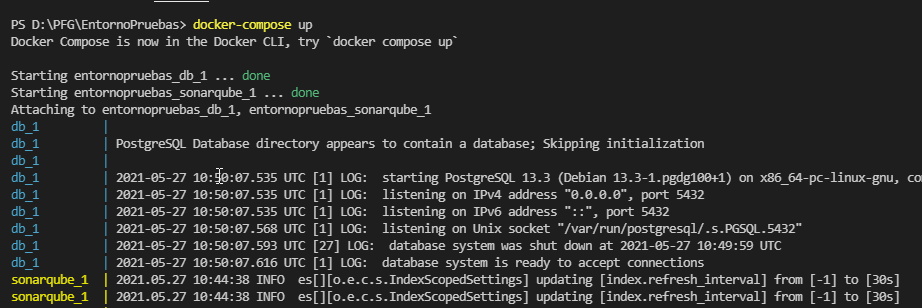
\includegraphics[width=\linewidth]{./imagenes/04_DockerCompose_UP.png}
    \caption{Docker compose up}  
\end{figure}

\clearpage
\newpage
Una vez que se veamos las siguientes líneas en el log:\\
\begin{figure}[!htb] 
    \captionsetup{width=1\linewidth}   
    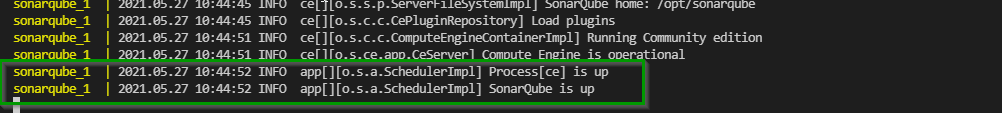
\includegraphics[width=\linewidth]{./imagenes/05_SonarQubeServerRunning.png}
    \caption{SonarQube server running}  
\end{figure}

Podremos acceder a la página de SonarQube en 
la url \href{http://localhost:9000}{http://localhost:9000}\\
\begin{figure}[!htb] 
    \captionsetup{width=1\linewidth}   
    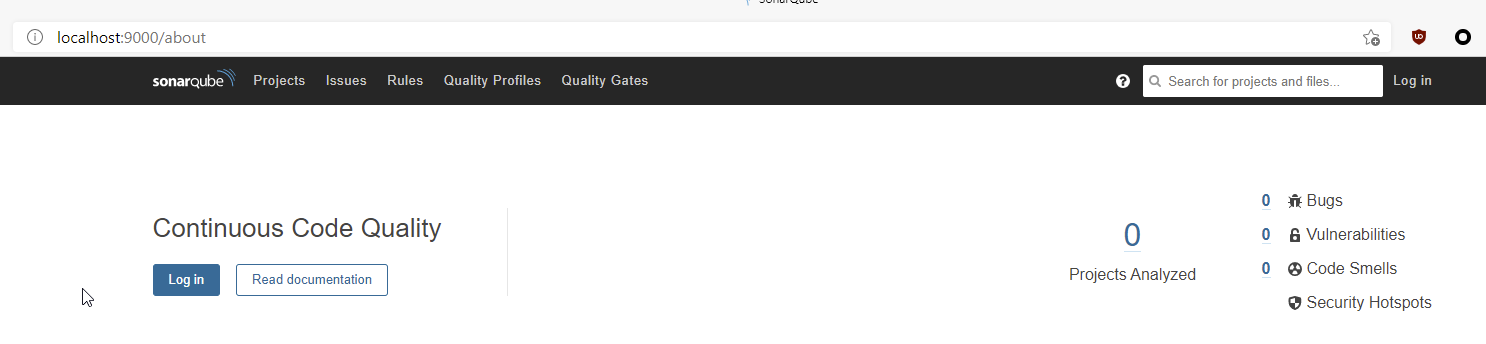
\includegraphics[width=\linewidth]{./imagenes/06_SonarQubeServer_Webpage.png}
    \caption{SonarQube portal}  
    \label{fig:21}
\end{figure}

\clearpage
\newpage
El fichero del docker compose \ref{alg:dockercompose} muestra los componentes de a aquitectura utilizados:

\begin{listing}
    \centering
    \inputminted{yaml}{./EntornoPruebas/SonarQube_8.2/docker-compose.yml}
    \caption{Docker Compose}
    \label{alg:dockercompose}
\end{listing}

\clearpage